\documentclass[conference]{IEEEtran}
\usepackage{cite}
\usepackage{amsmath,amssymb,amsfonts}
\usepackage{graphicx}
\usepackage{textcomp}
\usepackage{xcolor}
\usepackage{tabularx}
\usepackage{booktabs}
\usepackage{tikz}
\usetikzlibrary{shapes.geometric, arrows.meta, positioning, fit}

\begin{document}

\title{EdgeHealth: A Privacy-Preserving Edge Computing Gateway for Smartwatch Health Monitoring}

\author{
\IEEEauthorblockN{Nikhil Shankar}
\IEEEauthorblockA{
\textit{Computer and Information Science} \\
\textit{University of Michigan - Dearborn}\\
[Dearborn, Michigan] \\
[nikhilns@umich.edu]}
}

\maketitle

\begin{abstract}
Consumer smartwatches continuously collect sensitive health data---heart rate, blood oxygen saturation, and activity levels---yet transmit all raw readings to cloud servers for processing, raising significant privacy concerns and introducing latency in anomaly detection. We propose \textit{EdgeHealth}, an edge computing gateway that uses a Raspberry Pi to intercept and process smartwatch health data locally. The system receives real-time data from a Samsung Galaxy Watch via an Android relay application, performs hybrid anomaly detection (combining threshold rules with an Isolation Forest model) directly on the edge device, and transmits only aggregated daily summaries to the cloud. This architecture achieves privacy by design---raw health data never leaves the local network---while enabling sub-second anomaly alerts without cloud dependency. We evaluate the system on end-to-end latency, bandwidth reduction, detection accuracy, and resource utilization on the Raspberry Pi, comparing against a cloud-only baseline.
\end{abstract}

\begin{IEEEkeywords}
edge computing, health monitoring, anomaly detection, privacy, Raspberry Pi, smartwatch, Internet of Things
\end{IEEEkeywords}

\section{Problem Statement}

Wearable health devices such as the Samsung Galaxy Watch, Apple Watch, and Fitbit continuously monitor physiological signals including heart rate (HR), blood oxygen saturation (SpO\textsubscript{2}), and physical activity. The global wearable medical device market is projected to exceed \$30 billion by 2026, reflecting the growing reliance on continuous health monitoring~\cite{wearable_market}.

Currently, these devices follow a \textit{cloud-first} architecture: raw sensor data is transmitted from the wearable to the manufacturer's cloud servers (e.g., Samsung Health Cloud, Apple HealthKit Cloud) for storage and analysis. This design introduces three critical problems:

\textbf{Privacy exposure.} Intimate health data---resting heart rate patterns, sleep stages, SpO\textsubscript{2} fluctuations---is stored on third-party servers indefinitely. Users have limited control over how this data is used, shared, or retained. Health data breaches affected over 133 million records in 2023 alone~\cite{hipaa_breaches}.

\textbf{Latency in anomaly detection.} Cloud-based analysis requires a round trip: data upload, server-side processing, and alert delivery. This introduces delays of 3--10 seconds under normal conditions and becomes unreliable during network congestion or outages---precisely when timely health alerts may be most critical.

\textbf{Network dependency.} Cloud-only systems cease to function when internet connectivity is unavailable, leaving users without health monitoring during travel, rural stays, or network outages.

These problems motivate an \textit{edge-first} approach where health data is processed locally, alerts are generated immediately, and only minimal summaries reach the cloud. This benefits individuals who want continuous health monitoring with full data ownership, as well as scenarios requiring offline-capable or low-latency health awareness.

\section{System Design}

\subsection{Architecture Overview}

EdgeHealth consists of four components connected in a linear pipeline, as shown in Fig.~\ref{fig:architecture}:

\begin{figure}[htbp]
\centering
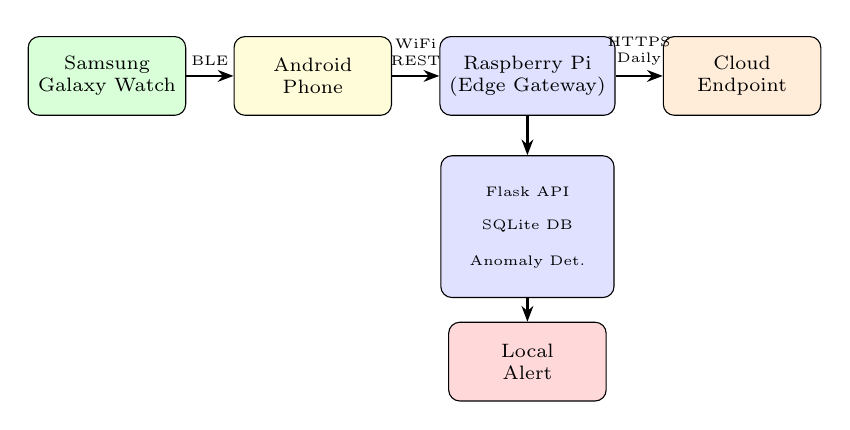
\begin{tikzpicture}[
    node distance=0.4cm and 0.6cm,
    block/.style={rectangle, draw, rounded corners, minimum height=1.0cm, minimum width=2.0cm, align=center, font=\scriptsize},
    edge_block/.style={block, fill=blue!12},
    cloud_block/.style={block, fill=orange!15},
    arrow/.style={-{Stealth[length=2mm]}, thick},
    label_style/.style={font=\tiny, align=center}
]

% Nodes
\node[block, fill=green!15] (watch) {Samsung\\Galaxy Watch};
\node[block, fill=yellow!15, right=of watch] (phone) {Android\\Phone};
\node[edge_block, right=of phone] (pi) {Raspberry Pi\\(Edge Gateway)};
\node[cloud_block, right=of pi] (cloud) {Cloud\\Endpoint};

% Sub-components of Pi
\node[edge_block, below=0.5cm of pi, minimum width=2.2cm, minimum height=1.8cm] (pi_detail) {};
\node[font=\tiny, align=center] at ([yshift=0.45cm]pi_detail.center) {Flask API};
\node[font=\tiny, align=center] at ([yshift=0.0cm]pi_detail.center) {SQLite DB};
\node[font=\tiny, align=center] at ([yshift=-0.45cm]pi_detail.center) {Anomaly Det.};

% Alert node
\node[block, fill=red!15, below=0.3cm of pi_detail] (alert) {Local\\Alert};

% Arrows
\draw[arrow] (watch) -- node[above, label_style] {BLE} (phone);
\draw[arrow] (phone) -- node[above, label_style] {WiFi\\REST} (pi);
\draw[arrow] (pi) -- node[above, label_style] {HTTPS\\Daily} (cloud);
\draw[arrow] (pi) -- (pi_detail);
\draw[arrow] (pi_detail) -- (alert);

\end{tikzpicture}
\caption{EdgeHealth system architecture. Health data flows from the smartwatch through the Android relay to the Raspberry Pi edge gateway. Only daily summaries are transmitted to the cloud.}
\label{fig:architecture}
\end{figure}

\textbf{(1) Samsung Galaxy Watch} (data source): Continuously collects HR, SpO\textsubscript{2}, step count, and sleep stage data. Syncs automatically to the paired Android phone via Bluetooth Low Energy (BLE).

\textbf{(2) Android Relay Application} (bridge): A custom Kotlin application reads health data from the Android Health Connect API every 60 seconds using a foreground service. New readings are serialized as JSON and transmitted to the Raspberry Pi over the local WiFi network via HTTP POST.

\textbf{(3) Raspberry Pi Edge Gateway} (core processing): Receives data through a Flask REST API, stores it in a local SQLite database, and runs anomaly detection every 5 minutes. Detected anomalies trigger immediate local alerts (buzzer, LED, or push notification via ntfy.sh). A nightly scheduled task computes aggregated daily summaries.

\textbf{(4) Cloud Endpoint} (minimal storage): A lightweight Flask server hosted on Render.com's free tier receives only daily summaries---minimum, maximum, and mean HR; total steps; sleep duration; anomaly count---via HTTPS POST. No raw sensor data is ever transmitted.

\subsection{Edge vs.\ Cloud Responsibilities}

Table~\ref{tab:edge_cloud} delineates the responsibilities of each tier.

\begin{table}[htbp]
\caption{Edge vs.\ Cloud Task Distribution}
\label{tab:edge_cloud}
\centering
\footnotesize
\begin{tabularx}{\columnwidth}{lXX}
\toprule
\textbf{Function} & \textbf{Edge (Raspberry Pi)} & \textbf{Cloud} \\
\midrule
Data ingestion & Real-time (every 60s) & None \\
Storage & Full raw data (SQLite) & Summaries only \\
Anomaly detection & Hybrid ML + thresholds & None \\
Alerting & Immediate, local & None \\
Long-term trends & None & Daily summaries \\
\bottomrule
\end{tabularx}
\end{table}

Processing is placed at the edge for four reasons: (a) \textit{privacy}---raw physiological data never leaves the local network; (b) \textit{latency}---anomaly detection occurs within milliseconds of data arrival, without a cloud round trip; (c) \textit{reliability}---the system functions fully during internet outages; and (d) \textit{bandwidth efficiency}---transmitting one daily summary (\(\sim\)200 bytes) versus \(\sim\)1,440 raw readings per day (\(\sim\)115 KB) reduces uploaded data by over 99\%.

\subsection{Anomaly Detection}

We employ a hybrid two-layer detection approach:

\textbf{Layer 1: Threshold Rules.} Hard-coded medical boundaries trigger immediate critical alerts: HR $<$ 40 or $>$ 180 BPM at rest, SpO\textsubscript{2} $<$ 90\%, or data silence exceeding 10 minutes.

\textbf{Layer 2: Isolation Forest.} A scikit-learn Isolation Forest model trained on normal activity data from the PPG-DaLiA dataset~\cite{ppg_dalia} identifies statistical anomalies that fall within safe thresholds but deviate from learned patterns. Features include instantaneous HR, HR rate-of-change ($\Delta$HR), step rate, and hour of day. The model operates on a sliding window of the 10 most recent readings and uses a contamination parameter of 0.05.

This hybrid approach balances safety (thresholds catch life-threatening values) with sensitivity (Isolation Forest catches subtle deviations).

\section{Implementation Plan}

\subsection{Key Features}
\begin{itemize}
    \item Real-time data ingestion from Samsung Galaxy Watch via Health Connect API
    \item Local anomaly detection with hybrid ML and threshold-based approach
    \item Instant local alerts with zero cloud dependency
    \item Privacy-preserving daily summary transmission to cloud dashboard
    \item Full offline operation capability
\end{itemize}

\subsection{Tools and Technologies}
\textbf{Hardware:} Raspberry Pi 4/5, Samsung Galaxy Watch, Android smartphone.
\textbf{Edge software:} Python 3.11, Flask, SQLite, scikit-learn, pandas, APScheduler, psutil.
\textbf{Mobile:} Android (Kotlin), Health Connect client library, OkHttp.
\textbf{Cloud:} Flask on Render.com (free tier).
\textbf{Dataset:} PPG-DaLiA~\cite{ppg_dalia} for model training and evaluation.

\subsection{Feasibility and Scope}

The project is scoped for approximately 45 hours over six weeks: environment setup and data pipeline (Week~1), Android relay application (Week~2), anomaly detection model training and deployment (Week~3), alerting and cloud integration (Week~4), evaluation and measurement (Week~5), and paper writing (Week~6). Fallback strategies include using Samsung Health CSV exports or the PPG-DaLiA dataset if real-time Health Connect access proves challenging.

\section{Evaluation Plan}

The system will be evaluated using six quantitative metrics, compared against a cloud-only baseline where all raw data is transmitted for remote processing.

\begin{table}[htbp]
\caption{Evaluation Metrics}
\label{tab:eval}
\centering
\footnotesize
\begin{tabularx}{\columnwidth}{lXl}
\toprule
\textbf{Metric} & \textbf{Method} & \textbf{Target} \\
\midrule
End-to-end latency & Timestamps at each pipeline stage & $<$ 2\,s \\
Inference latency & Timer around model prediction & $<$ 50\,ms \\
Bandwidth reduction & Raw bytes vs.\ summary bytes/day & $>$ 90\% \\
CPU utilization & \texttt{psutil} logging on Pi & $<$ 15\% \\
Memory usage & RSS measurement via \texttt{psutil} & $<$ 100\,MB \\
Detection accuracy & Precision/Recall/F1 on PPG-DaLiA & P $>$ 0.80 \\
\bottomrule
\end{tabularx}
\end{table}

The evaluation protocol involves replaying 24 hours of PPG-DaLiA data through the full pipeline while logging all metrics. We will compare three detection configurations---threshold-only, Isolation Forest-only, and hybrid---and contrast the edge architecture against the cloud-only baseline on latency and bandwidth. Results will be presented as latency histograms, bandwidth bar charts, resource utilization time series, and a precision-recall analysis.

\begin{thebibliography}{00}
\bibitem{wearable_market} Fortune Business Insights, ``Wearable Medical Devices Market Size, Share \& Industry Analysis,'' 2024.
\bibitem{hipaa_breaches} HIPAA Journal, ``Healthcare Data Breach Statistics,'' 2024.
\bibitem{ppg_dalia} A.~Reiss, I.~Indlekofer, P.~Schmidt, and K.~Van~Laerhoven, ``Deep PPG: Large-scale heart rate estimation with convolutional neural networks,'' \textit{Sensors}, vol.~19, no.~14, 2019.
\end{thebibliography}

\end{document}
